\chapter{Security Challenges in Smart Constracts}
\markboth{Security Challenges in Smart Constracts}{}
\chaptauthors{Lucas Pelloni and Ile Cepilov}

\Kurzfassung{%
%Gli Smart Contract oggi giorno rappresentano una valida alternativa a contratti tradizionali %e possono automatizzare l'agreement di termini legali tra più parti. 
%La loro efficacia è garantita sia da una solida piattagorma sulla quali essi vengono %eseguiti, sia da una nuova tecnologia sempre più in ascesa come la Blockchain. 
%Tuttavia, nonostante gli sforzi degli sviluppatori di scrivere codice sicuro e "impenetrabile" agli occhi degli hackers, si sono verificati nel corso degli ultimi tempi numerosi attacchi hacker, che hanno evidenziato diverse falle all'interno del codice di questi contratti. 
%L'impiego degli Smart Contract all'interno della vita quotidiana appare ancora lontano. Sia a a causa di una diffusione ancora di nicchia della sopracitata Blockchain technology, che di un trade-off tra il "fidarsi di una softaware o di una persona". 
It fits pretty much on one page and is definitely not longer.}

\newpage

\minitoc %table of contents

\newpage
%http://blockgeeks.com/guides/what-is-blockchain-technology/
%http://www.investopedia.com/terms/b/blockchain.asp
%https://letstalkpayments.com/an-overview-of-blockchain-technology
% PWC: PAPER DA PRENDERE ASSOLUTAMENTE http://www.pwc.ch/en/2017/pdf/pwc_blockchain_opportunity_for_energy_producers_and_consumers_en.pdf


\section{Blockchain Technology}
\subsection{Definition of Blockchain}
A blockchain is like a distributed database which constantly keeps a list of transaction or records, that have ever been executed, called usually blocks. Every record contains a reference to its predecessor and a timestamp \cite{wikipedia1}.
Data in a record cannot be changed due to its design. This makes them tampering-proof as well as a very good source of trust for the near future \cite{blockchain3}.
The blockchain works and is maintained by the entire community, which keeps and verifies all records and acts like a node of a peer-to-peer network, making the need of a thirty part trust organisation useless \cite{blockchain0}.
\subsubsection{Source of Trust}
A blockchain is based on a very powerful cryptographic concept. Original pieces of information are converted into code thanks to the application of a hash function. In this way, any attempt to attack it will result in a different hash value which will not allow any further modification.
%http://www.investopedia.com/terms/b/blockchain.asp
Thus, the blockchain might become a global decentralised source of trust \cite{blockchain3} for all parties involved in the business.\\
Usually, everything that is centralized is easy to attack because it offers a single point of failure (e.g. Firewall of a website). 
Applications built with Blockchain technology do not require users to trust developers with personal informations or funds \cite{blockchain3}, i.e. the need of an authority or an institution such as a bank,which acts as a middleman to make a transaction, is no longer needed. Moreover, buyers and sellers can directly transact with each other with the benefit of reducing the costs of transacting.
%https://www2.deloitte.com/nl/nl/pages/innovatie/artikelen/blockchain-technology-9-benefits-and-7-challenges.html
\section{Smart Contract: Introduction}
\subsection{Smart Contract: a self-executing contractual agreements}
%definition founded here: https://www.youtube.com/watch?v=FkeLDPZ-v8g&t=134s
A Smart Contract is a computer protocol (or piece of software) that includes, simplifies and verifies the negotiating terms for the execution of a contract. They do not contain a formal contract clause but they usually simulate it \cite{SC1}.
Smart Contracts are encrypted and implemented as programs running on the nodes of a custom public blockchain network, which is not the same used for Bitcoins transactions. Thanks to their encryption, an external trusted authority is no longer needed and thanks to the redundancy of the blockchain across the network, there will not be any loss of data or integrity in case of a system failure.
If a new Smart Contract has to be added to the blockchain, the miners, which are the actual nodes of the peer to peer network, have first to validate its execution and only once it has been validated by the majority of them, it can be actually appended to the blockchain \cite{SC2}.


%https://bitsonblocks.net/2016/02/01/a-gentle-introduction-to-smart-contracts/%
%http://www.businessdictionary.com/definition/legally-binding.html
\subsubsection{Traditional vs. Smart Contract}
A \textit{traditional contract} is normally an agreement, which consciously and legally bind two or more parties, who accept the terms and conditions contained inside the contract \cite{SC12,SC13}. For the execution of a \textit{traditional contract} there is always a need of a middleman (\textit{e.g. a lawyer}), who verifies and checks the agreed terms within the contract. However, this kind of a deal can imply excessive costs, may be prone to delays or might cause misunderstandings between the parties. 

           \begin{figure}[H]
         \begin{center}
         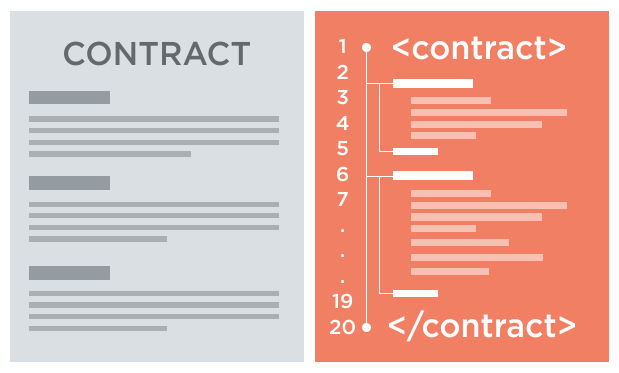
\includegraphics[scale=0.35]{Talk3/img/tradVSsmart}
         \end{center}
         \caption{A traditional vs. a Smart Contract, from \cite{SC2}.}
         \label{label}
       \end{figure}
cita\cite{SC2}






%1. As shown in the example, a smart contract is faster than a traditional one, which means that it can be executed faster

%2. The payment process can be executed automatically

%3. A Smart Contract is for sure cheaper than a traditional one. You don’t have to pay for a middleman who checks the agreements, you have only to pay the ”code”.

%4. A Smart Contract cannot get lost and its always available in chronological order on the blockchain for future access 

%Like said before, there is no need of a middleman (lawyer) 

\subsection{Smart Contracts and Blockchain technology}
           \begin{figure}[H]
         \begin{center}
         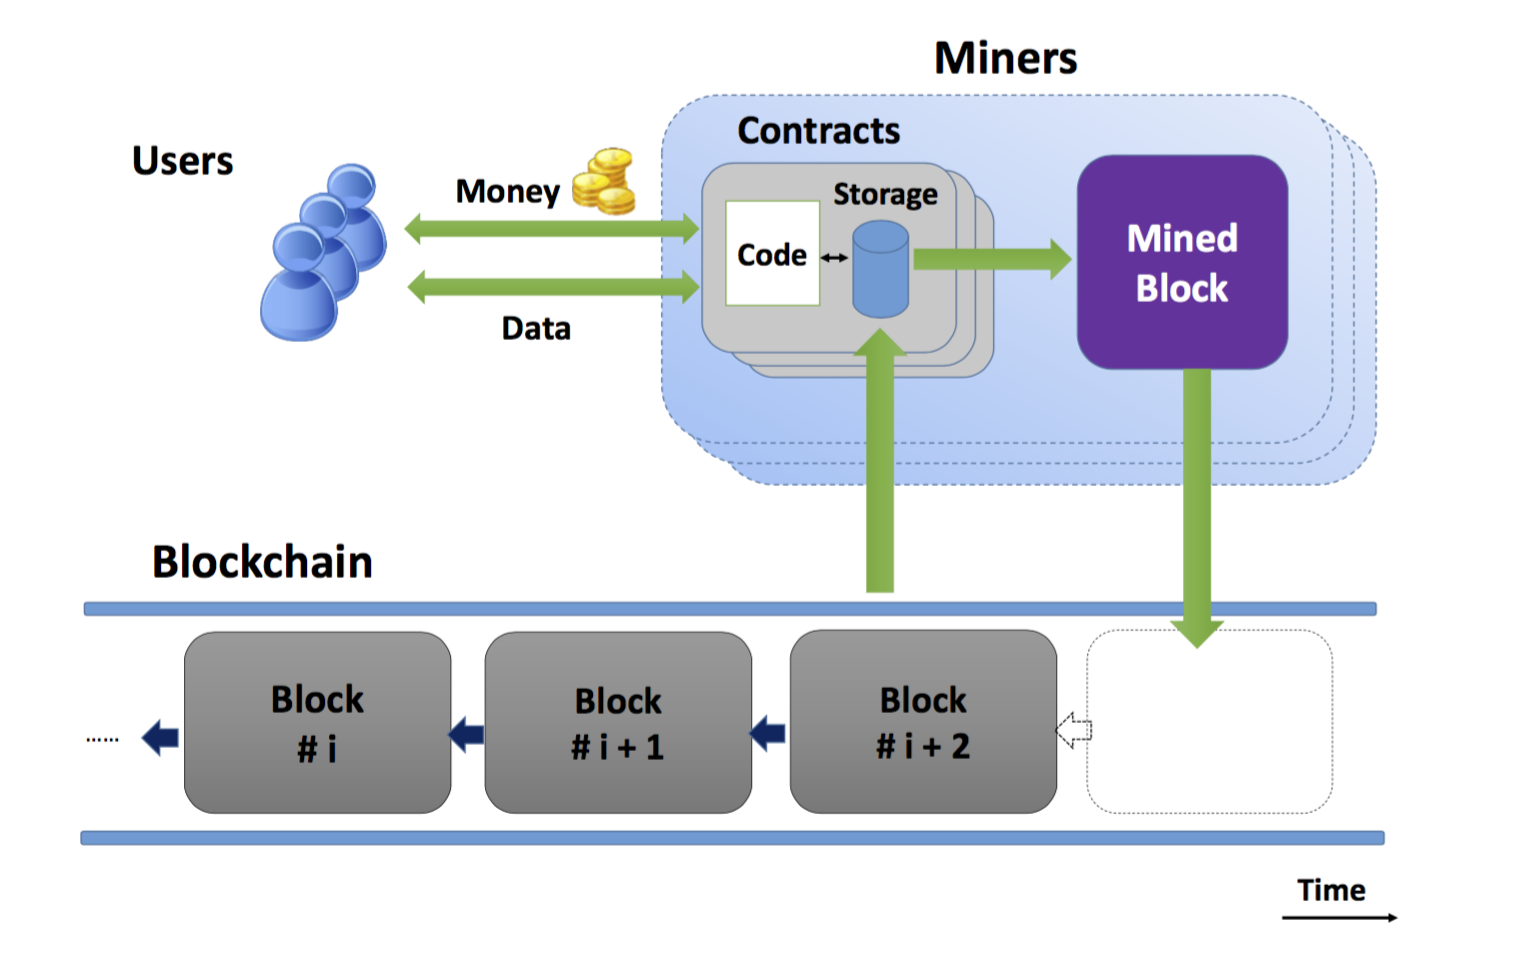
\includegraphics[scale=0.45]{Talk3/img/sc_blockchain}
         \end{center}
         \caption{Decentralized system with smart contracts, from \cite{paper3}}
         \label{label}
       \end{figure}

\subsection{Ethereum: a public blockchain-based platform}
Ethereum is a platform for the publication and the execution of Smart Contracts. It is decentralized \cite{paper2} and executes the Smart Contracts as programmed from their creator.
It has a own cryptovalue called Ether which is used as payment for the execution of Smart Contracts.
At the 24th of April 2017, the value of the currency compared to Bitcoins corresponded to 25 ETH to 1 BTC, which might not seem a lot but when compared to a fiat currency, like the swiss currency, it would correspond to circa 1242 CHF.\\
This high value of Bitcoins can be attributed to its monetary inflation from 2010 up until today (the 24th of May) \cite{BitcoinsPriceCharts}. Indeed, this currency growth, not being conditioned by macroeconomic factors (such as authorities), could not have been foreseen. \\
Ethereum's contracts are written in Solidity, which is an objected-oriented language programming language, similar to Java, and it is exclusively designed for coding Smart Contracts.
The Smart Contracts are then compiled in the Ethereum virtual machine (EVM bytecode) and deployed finally on the Ethereum blockchain \cite{paper2}. 

\subsection{Smart Contract's properties in Ethereum}
In this section we will have a look at the key components that can be found inside a Smart Contract.
A Smart Contract must always have a {\itshape contract address} 
%PAPER 633.pdf% asddd
which can be used to identify it. It may contain some amount of Ether (The virtual coin used in Ethereum) in its {\itshape balance} attribute.
\\It has a very important function which does not take any parameter at all, i.e. the so called {\itshape Fallback} function(). This function will be triggered by default when a contract is invoked by a transaction.
\\It is very important because, as we will see in the next sections, it has been exploited a lot in the most famous attacks.
\\Of course, some more informations have to be stored in it, like who the sender is, the amount of Ether that is sent to the contract and some more info for the transaction. All this data are saved in a variable {\textit msg.}
%http://www.coinfox.info/news/reviews/5195-ethereum-and-smart-contracts-in-depth
\\Now we would like to introduce the Gas system. The gas is used to express the cost of a computation done by the EVM, which in turn will be payed in the currency (Ether). Even though the actual currency may variate, the price of the network resources (Gas) stays constant.
\\The gas is divided in three main component, {\textit the Gas Cost, the Gas Price and the Gas Limit.}
\\The Gas Cost has a static value over time, whereas the Gas Price, measured in ether, changes accordingly to the cryptocurrency's fluctuation. But like we said before, the real cost of the Gas should remain the same, which means that an increase of the price of ether will have as a consequence a drop down of the Gas Price.
\\When somebody sends a transaction to invoke a contract, he has to specify hos much Gas he/she is willing to provide for its execution (Gas Limit). 
%To run a particular transaction or program (called “contract”), one has to pay an amount of Gas (called Gas %Fee) to miners. There is a list of fixed default fees for particular operations 




\subsubsection{Solidity: a typed JavaScript-like language}
TODO: CONTROLLARE LA VALIDITA 
As introduced in Ethereum, Solidity is a object-oriented programming language for writing smart contracts and it can be used on various blockchain even though it is used as the primary language on the Ethereum platform.
%https://en.wikipedia.org/wiki/Solidity
\\It was first proposed in August 2014 by Gavin Wood and developed later by the Ethereum project's Solidity team (CITA MEEENCHIA)

\section{Smart Contract attacks}
\subsection{DAO Attack}
\subsubsection{Attack description}
One of the most famous attack on Smart Contracts was the DAO Attack (Decentralised Autonomous Organisation)\cite{SC6}.
%https://www.wired.com/2016/06/50-million-hack-just-showed-dao-human/
The DAO was a crowd-funding project which, like traditional mutual funds, allows investors or "members" to purchase shares and enjoy returns based on its performance.
On 17 June 2016, the attacker managed to steal 3.6 Milion Ether\footnote{Corresponding to USD 60 million} from the Ethereum's platform and putting them into a personal account \cite{SC8}.\\ %http://www.clydeco.com/insight/article/ethereums-dao-attack-smart-contracts-and-blockchain-face-their-first-big-te
Due to the strong impact of this attack to the Etherum platform, the value of the Ether currency drastically dropped from 20.5 USD to 11.20 USD \cite{SC9}.  
%http://uk.businessinsider.com/dao-hacked-ethereum-crashing-in-value-tens-of-millions-allegedly-stolen-2016-6
). \\
We now consider only a streamlined version of the DAO attack, also called \textbf{SimpleDAO}, which is the first of the two known DAO attacks and has some common characteristics to the original one. The attack described below allows the hacker to siphon all the ether contained within the \textbf{SimpleDAO} Smart Contract \cite{paper2}. \\
The first thing the attacker has to do is to publish a \textbf{Mallory} Contract (as shown below): 
\begin{figure}[H]
\begin{center}
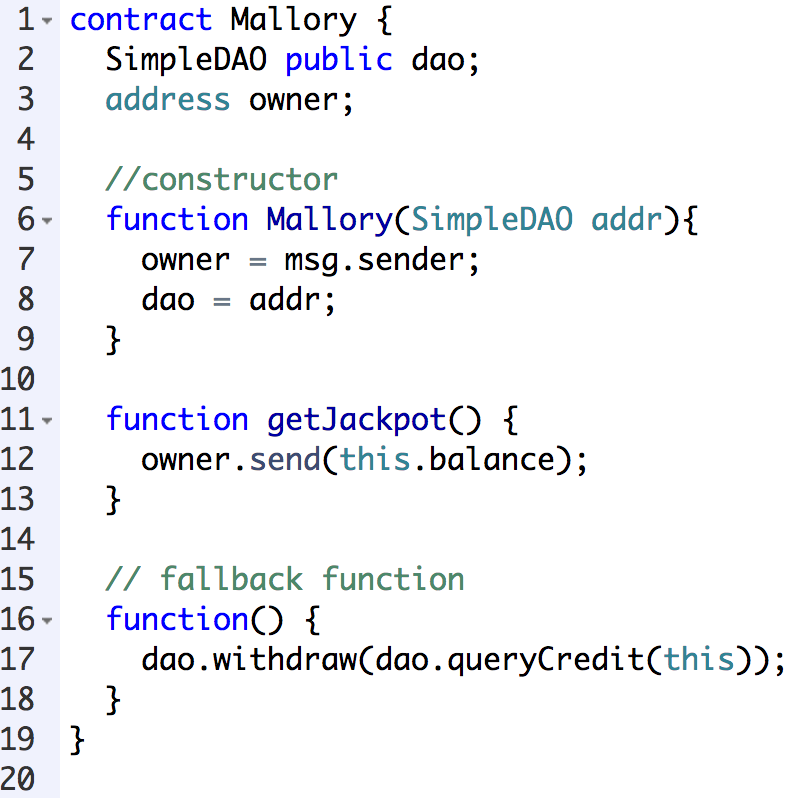
\includegraphics[scale=0.50]{Talk3/img/dao1}
\end{center}
\caption{Dao Attack: the Mallory contract}
\label{label}
\end{figure}
%https://github.com/chriseth/solidity-doc-test/blob/master/docs/frequently-asked-questions.rst
%http://solidity.readthedocs.io/en/latest/frequently-asked-questions.html
After publishing the contract, the hacker sends some Ether to Mallory and automatically invokes the Mallory Fallback\footnote{A Fallback is just a function without any name or parameter, which is called by default if some ether is sent to a contract \cite{SC10}. } (line 16, \textbf{Mallory}). \\
The \textbf{Mallory}'s fallback, in turn, calls the \textbf{withdraw} function written in the \textbf{SimpleDAO}\footnote{The whole Smart Contract's code is findable here: http://co2.unica.it/ethereum/attacks.html\#simpledao} contract (figure below), which is in charge of sending an amount of Ether to a specified public address. 
\begin{figure}[H]
\begin{center}
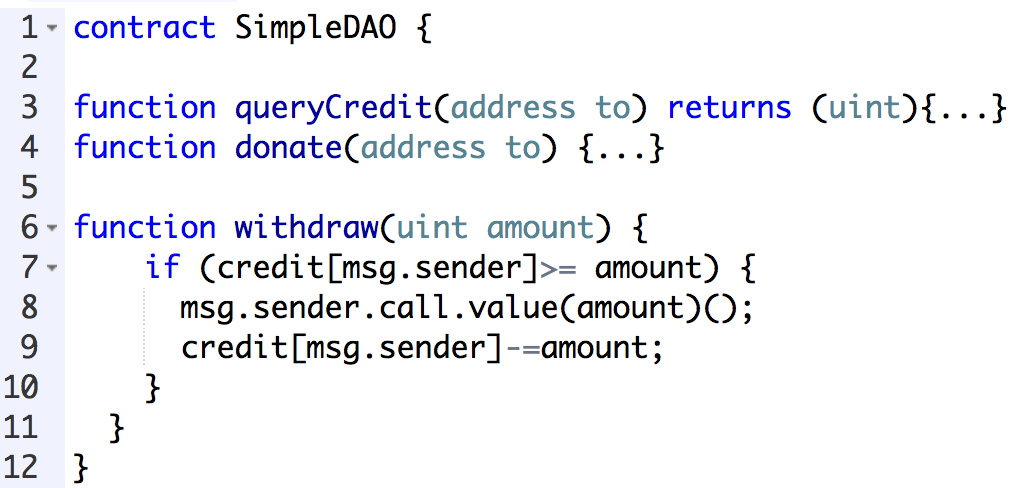
\includegraphics[scale=0.55]{Talk3/img/dao2}
\end{center}
\caption{Dao Attack: the SimpleDAO contract}
\label{label}
\end{figure}
Since the \textbf{withdraw} function of the \textbf{SimpleDAO} has been invoked by the \textbf{Mallory} fallback, it simply sends the Ether to Mallory (line 6, \textbf{SimpleDAO}). By sending the Ether to \textbf{Mallory}, the \textbf{Mallory}'s fallback gets invoked again. As a consequence, the \textbf{withdraw} function transfers the specified amount of Ether to \textbf{Mallory} for the second time. The flaw of this sequence of function calls resides at line 9 of the \textbf{SimpleDAO} contract, where the real amount of Ether stored within the contract gets never updated. 
This kind of loop goes on until one of the following conditions is satisfied: \\
\begin{enumerate}
%cita nella footnote: https://www.cryptocompare.com/coins/guides/what-is-the-gas-in-ethereum/
\item The gas is exhausted\footnote{Internal fee in Ethereum paid to the miners, proportional to their power computation\cite{SC11}}
\item Call Stack is full
\item Balance of DAO gets down to zero  
\end{enumerate}





\subsubsection{No solutions, only countermeasures}
Sadly, there was a lack of solutions for stopping this attack. The only possible choice was to suppress the attack and the community was faced with two of them.
\\A first choice was to do a {\textit Soft fork} which consisted in freezing the transaction that belonged to the attacker. But not the majority of the whole community agreed with it and more important, the transactions that were used by the attacker in order to move the stolen funds, would have ignored and not reverted and therefore the miners would not have been paid
\\Moreover, in doing so, a potential DOS attack would have been introduced. 
(cit:)
%https://steemit.com/crypto-news/@help-yourself/the-dao-soft-fork-solution-has-a-potential-dos-vector
Specifically, an attacker can flood the network with transactions that execute difficult computation, and end by performing an operation on the DAO contract. Miners running the soft fork would end up having to execute, and then subsequently discard, such contracts without collecting any fees.
\\Therefore a {\textit Soft fork} was proposed and approved on the 19th of July. Its intention was to put into a new refund Smart Contract all the ether taken by the attacker during the attack. The refund Smart Contract would have only one functions withdraw allowing the poor victims get back their stolen funds.
\subsection{MultiPlayer Attack}
The Multiplayer Attack is based on a game between two players. The rules are really simple, each player who joins the game has to chose a number, once both player have chosen a number, the sum of the number is calculated and if the result is even the first player wins, if the sum is odd the second one wins.
\\Now, let's have a closer look at the interesting part of the contract:
\begin{figure}[H]
\begin{center}
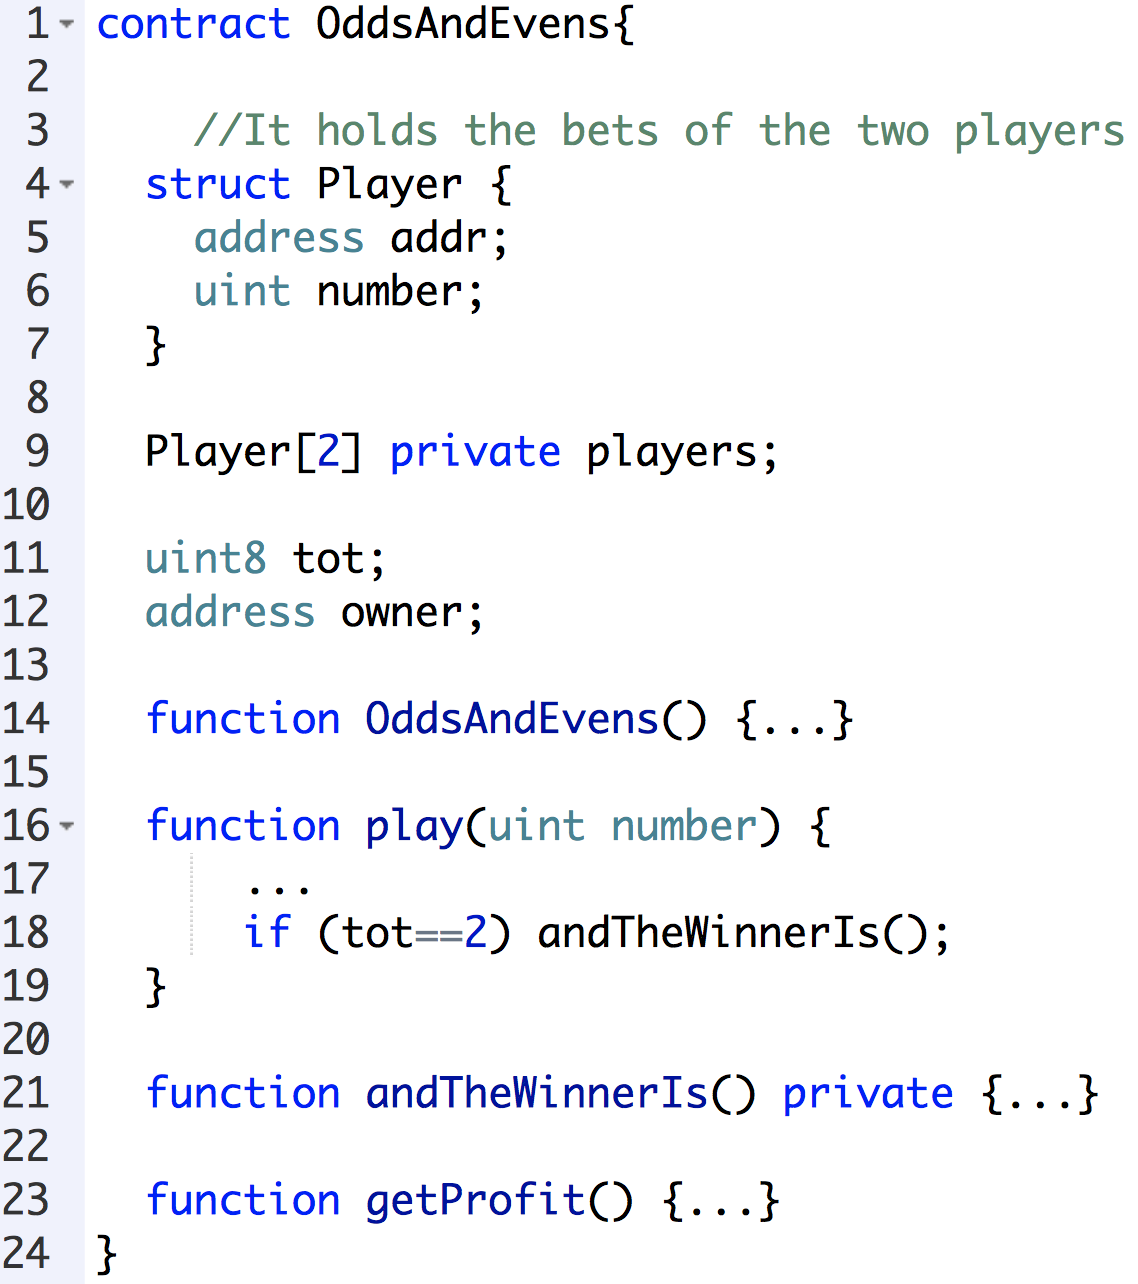
\includegraphics[scale=0.40]{Talk3/img/oae1}
\end{center}
\caption{Odd and Even contract}
\label{label}
\end{figure}
At line 4 we can see a struct that is used to hold the bets of the two players and at line 9 a private array stores them in a players variable. As you can see the array is declared as private, preventing other contract to directly read into it.\\
To join a game,  the function play at line 16 gets invoked and if all the omitted conditions inside are satisfied, an exception gets thrown and the amount is sent back to the player, otherwise the method at line 21 gets called, the winner is found and the new amount can be withdrawn by invoking getProfit().
\subsubsection{Attack description}
The attack is really simple and it does not require too much programming skills to be realized. As said in the description of the game, the array which holds the amount that has been bet by the two players is declared as private. This does mean that other contracts cannot ready its content, but it does not prevent an attacker from inspecting the transaction (the current state of the game) on the blockchain and actually see what is inside it. Once the attacker manages to inspect the blockain and check the other player's bet, he can play by betting a suitable amount in order to be the winner and withdraw the jackpot.
\subsubsection{Possible solution}
Since the blockchain is public, anyone can audit its content and making it private would go against the real purpose of the blockchain. In order to prevent these attacks, which exploit this kind of vulnerability, some techniques like Timmed-Commitments \cite{timmedCommitments1, paper2} can be applied.\\
This approach consists of simply setting a time period in which the other player has to play his move. If the opposing player does not play within the given interval, he will get a penalty.
\subsection{Rubixi Attack}
Rubixi \cite{rubixi1, rubixi2} in another game avaiable on \textit{Ethereum}. It implements a fraudalent scheme, also known as \textbf{Ponzi scheme} \cite{paper2}.
This scheme \cite{ponzi}, can also be viewed as a fraudalent investment operation. For instance, \textit{the scheme's owner} promises out-of-standards gains on a short-term period, often referring to non-existent mechanisms. \\ 
However, at the beginning only few investors will give confidence to the person, also due to the lack of previously non-documented investments. 
For the few who will invest their money, the scheme's owner will keep his promise complying with the terms of the agreement. In doing so, the first investors will be recompensed with a very high ROI \footnote{Return Of Investment} and as consequence the scheme's owner will be able to benefit from her reputation to increase the invested capital and the number of investors. \\
The first participants, who have been repaid, will reinvest their money and will attract new victims into the scheme, telling them how much profitable is this kind of investment. \\
The money invested from the newcomers, will be used to pay the fees of the other participants and as soon as the scheme's owner reaches the maximum gains, he will disappear leaving the game. \\
\subsubsection{Attack description}
The suffered attack by \textit{Rubixi} was quite naive. During the development phase the game's name was changed from \textit{DynamicPyramid} into \textit{Rubixi}. \\
Unfortunately, game developers forgot to adapt the constructor name of the contract, which quickly became a public bug \cite{paper2}. \\
The figure below shows a simplified rappresentation of the bug mentioned above \cite{paper2}.

\begin{figure}[H]
\begin{center}
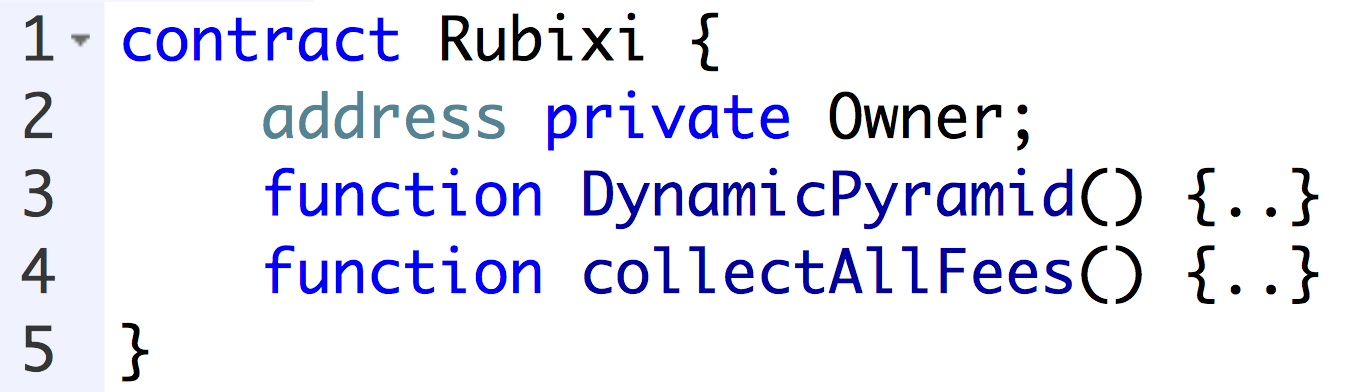
\includegraphics[scale=0.30]{Talk3/img/rubixi}
\end{center}
\caption{Faulty Rubixi contract}
\label{label}
\end{figure}

Users could just invoke the faulty \textit{DynamicPyramid} constructor and so they get associated as owners of the contract. After that, they could just withdraw the fees keep by the contract \cite{rubixi1}. 

\subsubsection{Possible solution}
The only obvious solution was to change the name of the constract from \textit{DynamicPyramid} into \textit{Rubixi}.

%sito originale: https://www.kingoftheether.com
%Post mordem: https://www.kingoftheether.com/postmortem.html
%source code: https://github.com/kieranelby/KingOfTheEtherThrone/blob/v0.4.0/contracts/KingOfTheEtherThrone.sol

\subsection{King of The Ether Throne}
The "King of the Ether" (or "King of the Ether Throne") is an Ethereum contract, stored on the blockchain, which implements a very simple game. cita: % https://www.kingoftheether.com 
The game's goal is to become the "King/Queen of the Ether". In order to make that possible, a player who wants to join the game has to pay an amount of Ether greater that the current claimprice. If the amount is greater, this player becomes the new King and a small fee has to be computed and paid to the old king. 
When a new King gets crowned, the claimprice is calculated and set as new prize of the game. The prize logically increases each time a new king is crowned \cite{paper2}. \\

\subsubsection{First Attack description}
For a proper explanation of this attack, consider the following \textbf{KotET} contract, which implements a simplified version of the original contract\footnote{the whole code can be found here: http://co2.unica.it/ethereum/attacks.html\#kotet}.   
\begin{figure}[H]
\begin{center}
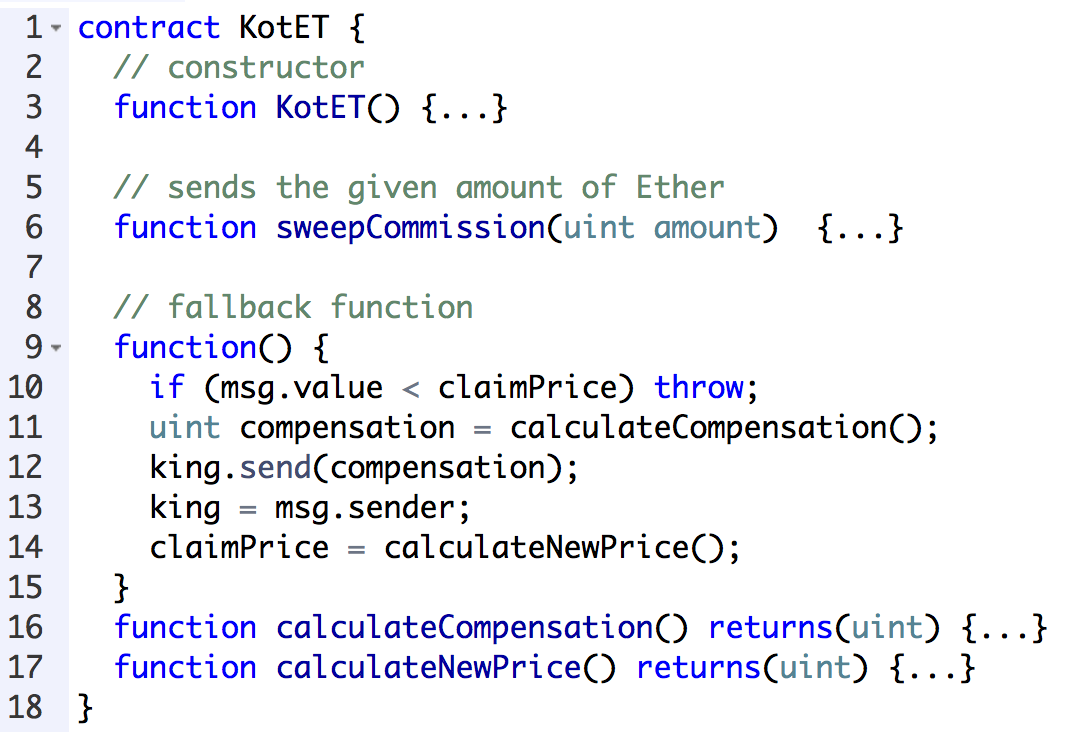
\includegraphics[scale=0.55]{Talk3/img/kot}
\end{center}
\caption{First KotET contract}
\label{label}
\end{figure}
Whenever a new player sends some Ether to the \textbf{KotET} contract, the fallback function gets invoked by default (line 9). The first "if-statement" inside the fallback function checks whether the sent Ether is greater that the current claimprice, otherwise an exception gets thrown and the whole transaction gets reverted. If the amount is enough, the compensation for the old king is computed and sent to him (line 11, 12). After that, the current player is crowned as new king and the new prize is calculated and stored inside the contract\cite{paper2}. \\
The flaw exploited in this attack resides at line 12. For this contract doesn't exist a control in the \textbf{return code} of the \textbf{send} function (cita) %da citare http://co2.unica.it/ethereum/attacks.html\#kotet 
and this may cause a lost of Ether.
If there would be someone, who wants to attack this contract, he could require much more gas for the \textbf{send} compensation function (which means, that his \textbf{fallback} function would be very expensive) (cita quello sopra). Indoing so, the function call at line 12 may fail and since there is no check in the return code (the \textbf{send} does not cause any exception) the compensation for the old king will thus remain by the contract, even in the case of a new crowned king. 
After that, the attacker could easily withdraw the compensation accumulated in the contract (via \textbf{sweepCommission}, at line 6).  

%cita questo: https://www.kingoftheether.com/contract-safety-checklist.html
\subsubsection{Possible solution}
The solution adapted by Ethereum to avoid future attacks is also known as the "failed sends" solution (cita). It consists of an attachment of a reasonable amount of gas with each transaction involving two or more parties (cita ancora). 
For example, if a miner would have a very expensive fallback function, an exception should be thrown and the whole transaction should be reverted. \\ For testing the accuracy of this solution Ethereum runned several functional tests\footnote{the simulated test cases described in the Ethereum on-chain report can be found here: https://github.com/kieranelby/KingOfTheEtherThrone/blob/v1.0/tests/onchain-test-report.md}, trying to cover the largest number of possible scenarios. 


\subsubsection{Second Attack description}
For making our explanation easier to understand, consider also in this case the following semplified \textbf{KotET} contract: 
\begin{figure}[H]
\begin{center}
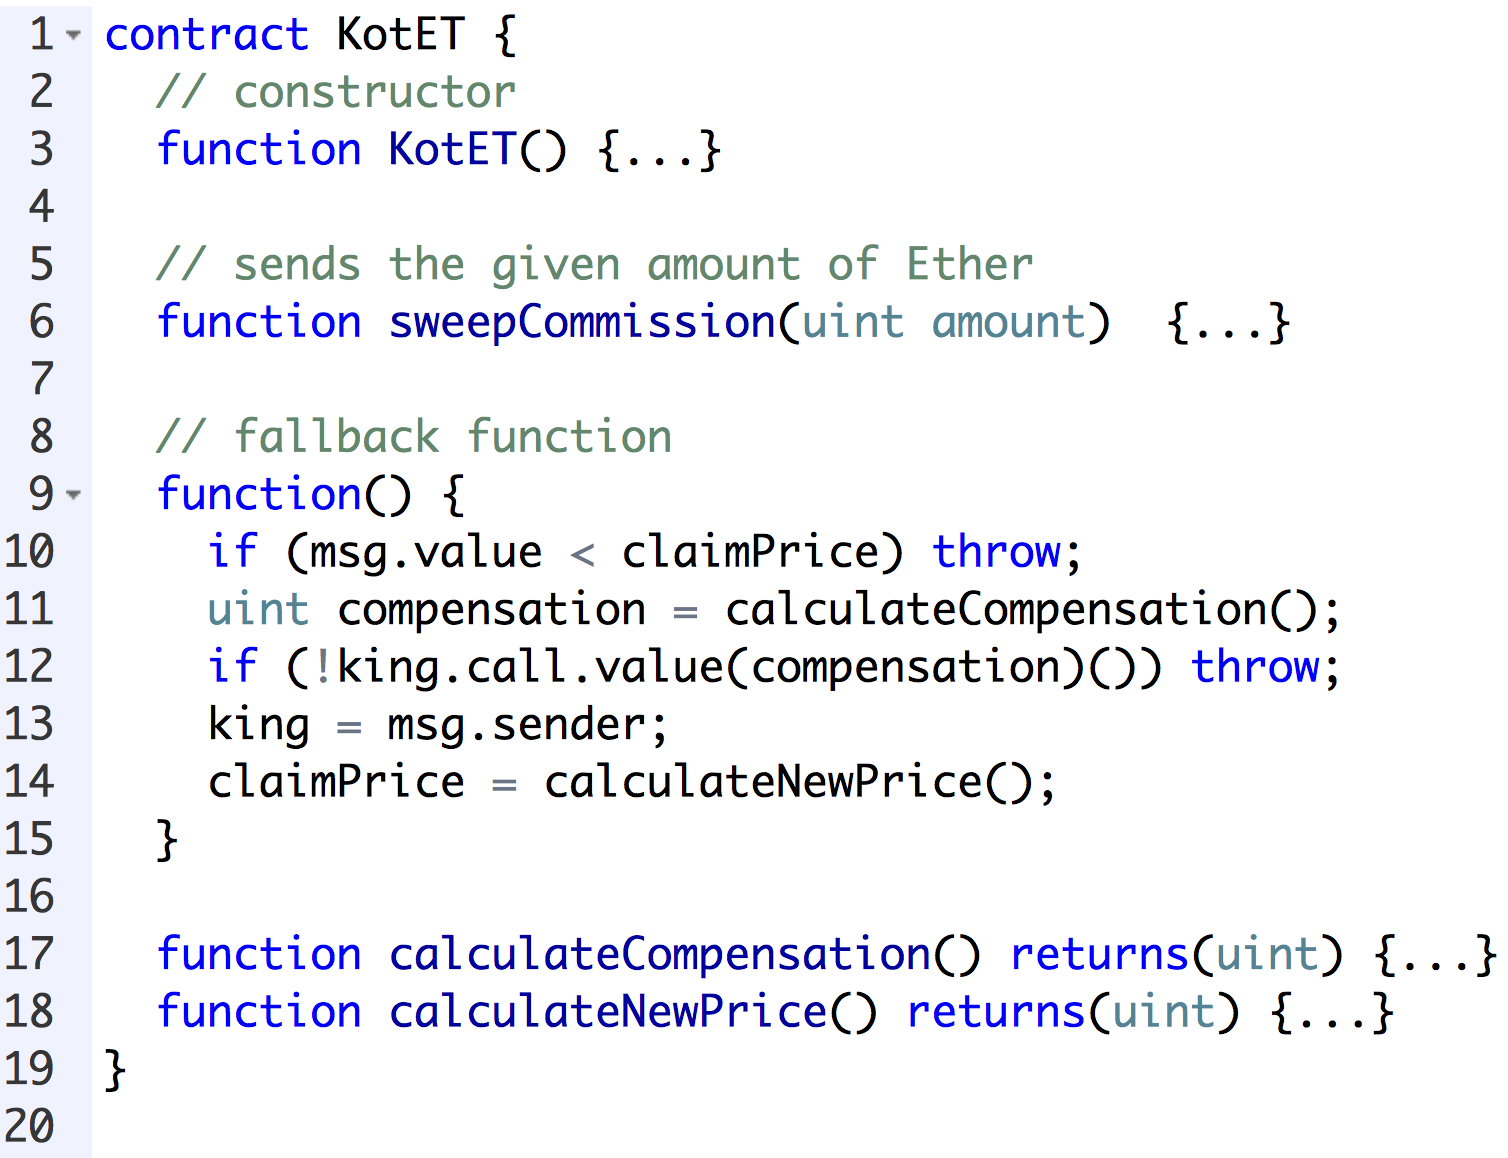
\includegraphics[scale=0.35]{Talk3/img/kot2}
\end{center}
\caption{Second KotET contract}
\label{label}
\end{figure}
As highlighted in the contract above, the only difference between the first KotET contract (mentioned in the paragraph above) and this contract resides in the \textbf{fallback function}, more specifically in the method with whom the compensation is sent to the old king. Indeed, the first contract implements a \textbf{send function}, while the second one uses a \textbf{call function} for transfering an amount of Ether. A \textbf{send} function is usually equipped with some gas\footnote{normally 2300 gas}, while a \textbf{call function} does not use any gas (cita). 
%difference between call/send: https://ethereum.stackexchange.com/questions/6470/send-vs-call-differences-and-when-to-use-and-when-not-to-use
Moreover, the second contract checks the return code of the \textbf{call} function and even though it should be more reliable that the first one, it can be also hacked. \\
Let's suppose that there would be someone, who wants to attack this contract publishing the following \textbf{Mallory} contract: 
\begin{figure}[H]
\begin{center}
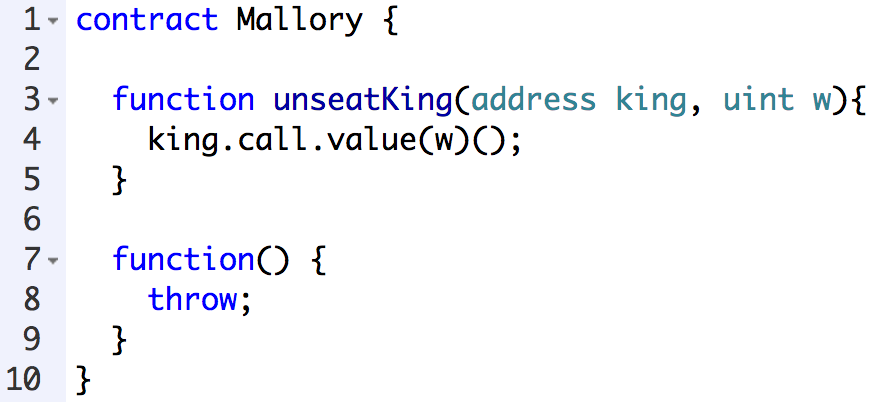
\includegraphics[scale=0.5]{Talk3/img/kot_mallory}
\end{center}
\caption{The KotET Mallory contract}
\label{label}
\end{figure}

This contract Mallory has a fallback, which just throws an exception. The hacker calls \textbf{unseatKing} with the right amount of Ether, so that Mallory becomes the new king. 
At this point, nobody else can get her crown, since every time \textbf{KotET} tries to send the compensation to Mallory, her fallback throws an exception, preventing the coronation to succeed. 

\subsubsection{Possible solution}
A way to solve this attack is to handle exceptions in an uniformly way. This means, that if the fallback function raises an exception the \textbf{whole transaction} must \textbf{always }be reverted and not only a sequence of nested calls \cite{paper2} between two functions. An unequal treatment in handling exception may cause attacks for smart contracts and we can conclude, in accord to a quantitative analysis published on \cite{anal}, that 28\% of Smart Contracts don't check the return code of \textbf{call/send} functions. 

\subsection{Govern-Mental: Introduction}
Govern-Mental is once again based on the ponzi scheme explained before. But before getting into the attack, we will explain you how this scheme works in this case.\\
To take part in it, a participant must send a  certain amount of ether to the contract. When nobody joins it for at least twelve hours, the last contributor is going to take all the ether contained in the contract, except of course for a small fee which is going to be kept by the owner of the contract.
Once the timer on the jackpot runs out, the two arrays are cleared as follows \cite{paper2}:
\begin{figure}[H]
\begin{center}
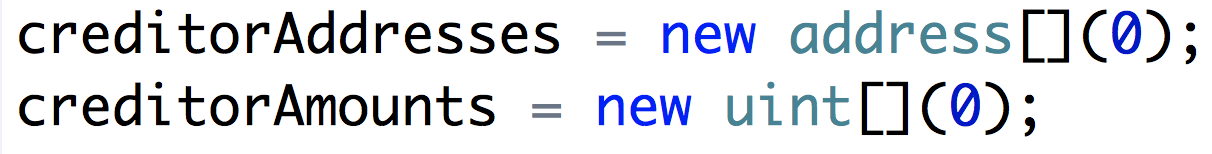
\includegraphics[scale=0.30]{Talk3/img/Governmental1Array}
\end{center}
\caption{Clearing the two arrays}
\label{label}
\end{figure}
A problem that arose had to do with the size of the two arrays. At some point the list got too big and the amount of ether required for clearing it was exceeding the maximum amount allowed for a single transaction. From then on, any endeavor in clearing them was useless.
To better understand the attacks that will come, we are first going to introduce you a simplified example of the contract:
\begin{figure}[H]
\begin{center}
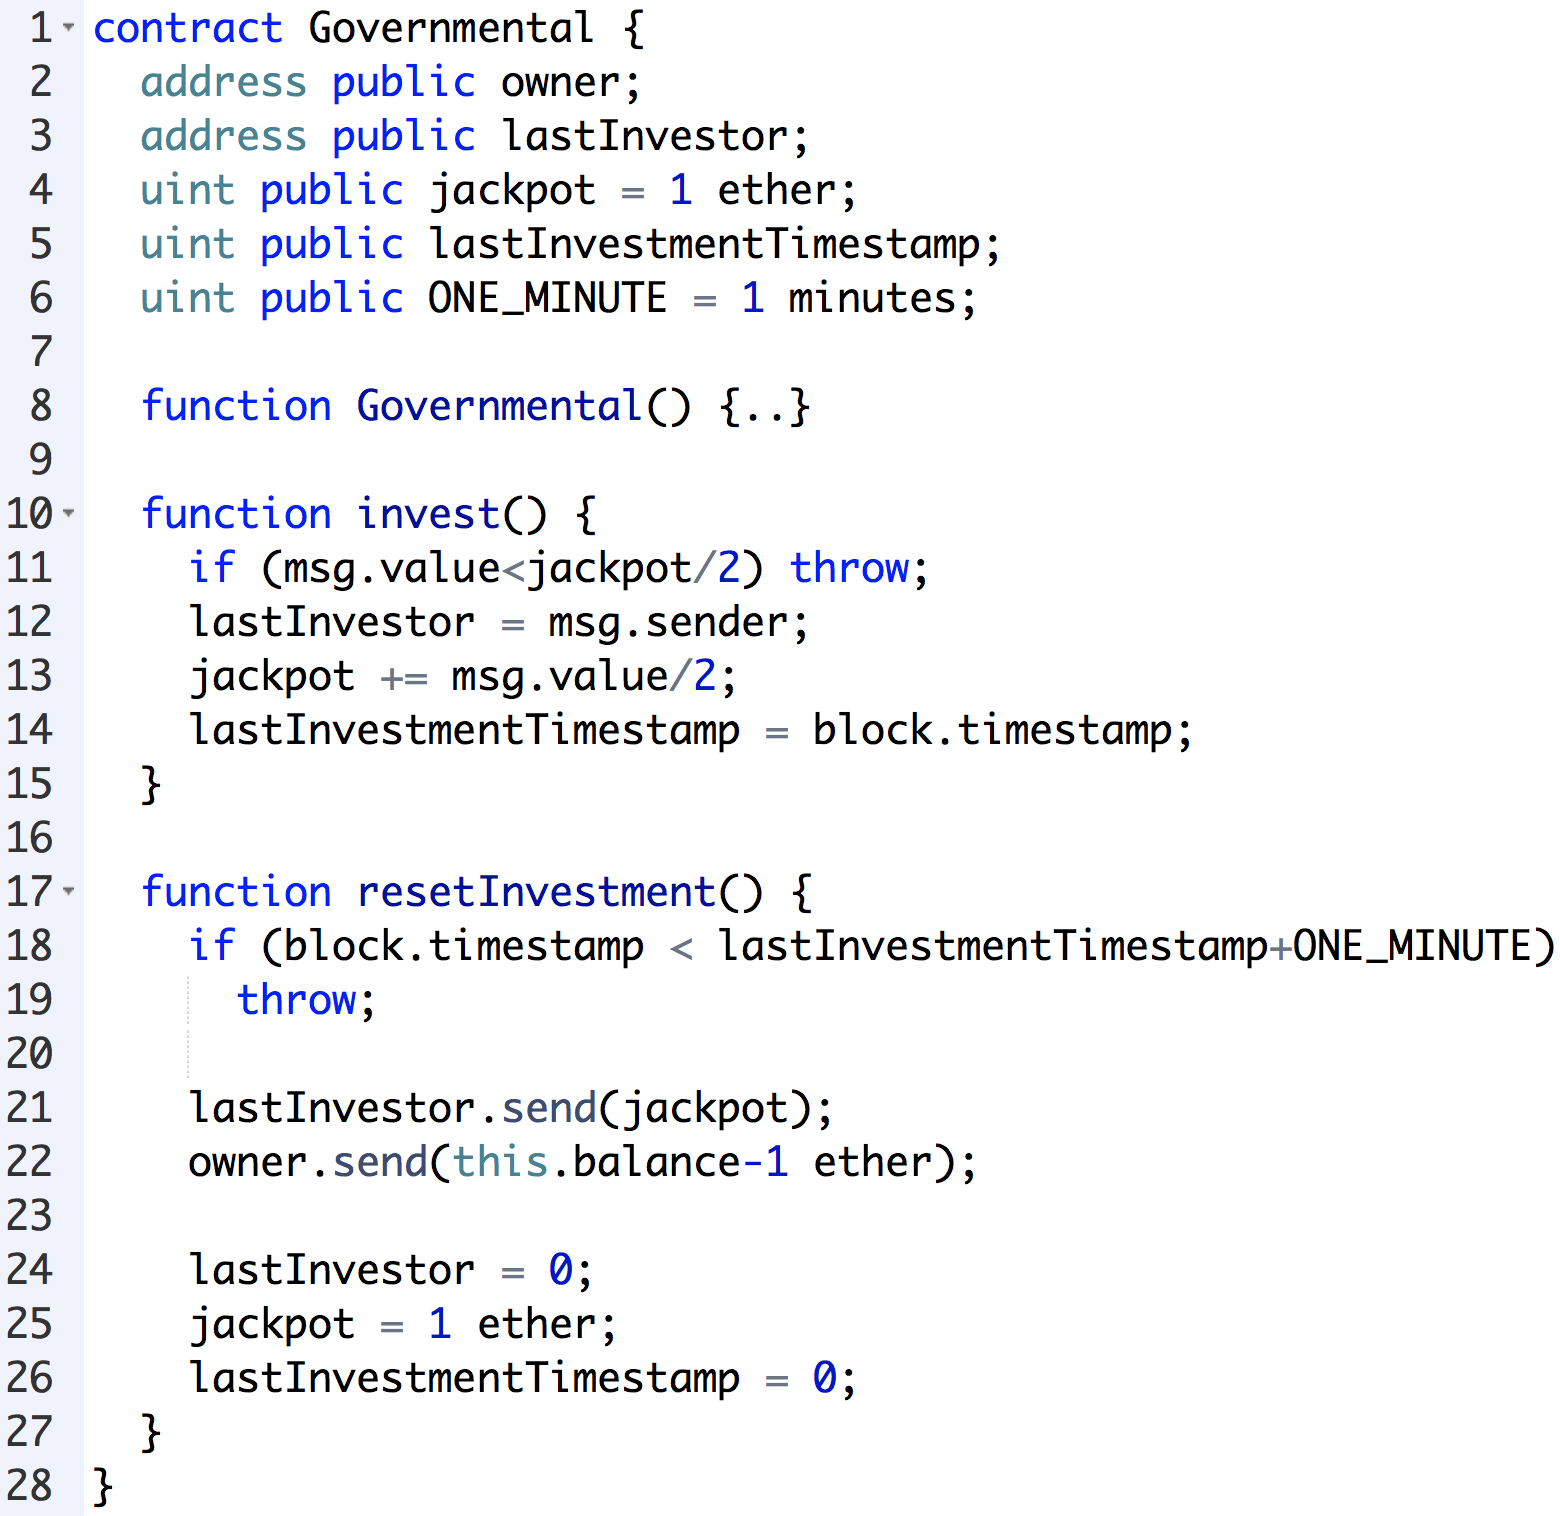
\includegraphics[scale=0.35]{Talk3/img/GovernmentalContract}
\end{center}
\caption{Clearing the two arrays}
\label{label}
\end{figure}
The Governmental contract takes the investments and it pays back only the player who is the last for at least one minute. A player must invest at least half of the jackpot (line 13), which grows with each new investment, to join the scheme. Anyone can invoke \textit{resetInvestment()}, which pays the half of the invested total (the jackpot) to the winner (line 17), and sends as usual the remaining ether to the owner of the contract.
\subsection{Govern-Mental: First Attack}
This first attack consists in keeping all the ether of the scheme in the contract. To achieve this intent, the send function (line 22) has to fail so that the real winner never gets back his money (the jackpot).
Obviously, the attacker in this case is going to be the owner of the contract because at the end he can take all the money.
The first thing to do is to publish an Attack contract like the following one:
\begin{figure}[H]
\begin{center}
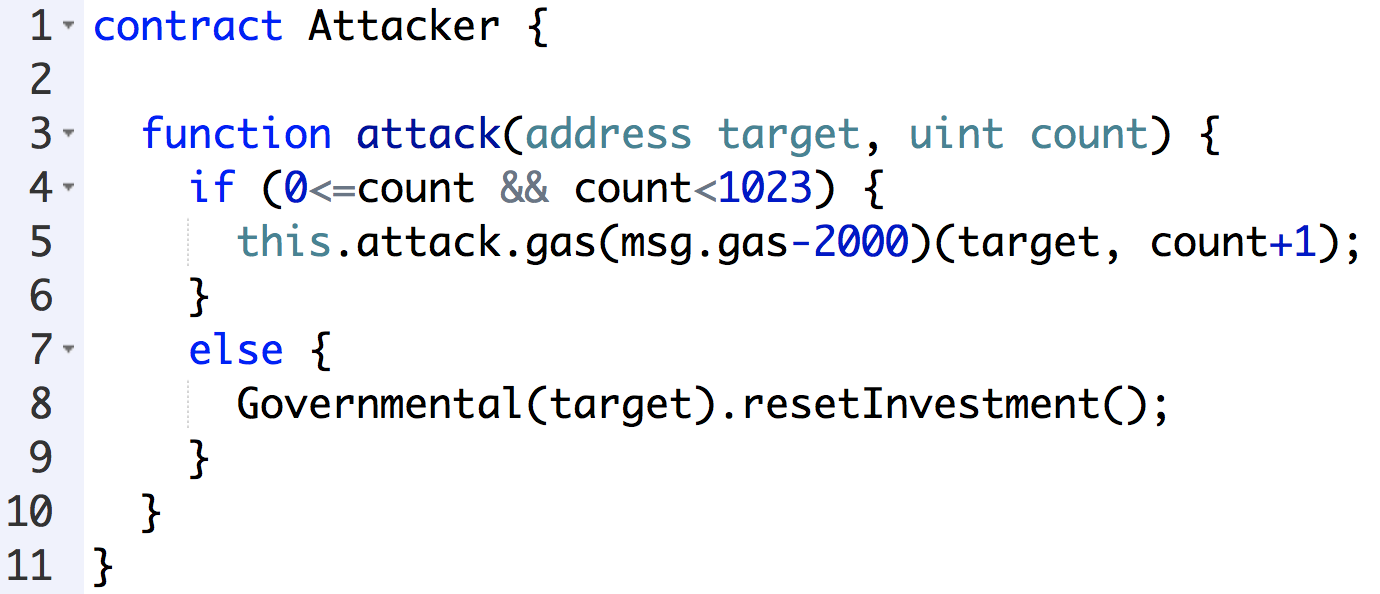
\includegraphics[scale=0.35]{Talk3/img/GovernmentAtttackContract}
\end{center}
\caption{Attacker contract}
\label{label}
\end{figure}
As you can see at line 5, the Attacker contracts starts recursively executing itself, increasing the stack of one frame at each call \cite{paper2}.
When the stack has grown enough (right before reaching the 1024 size) the \textbf{resetInvestment()} function in the else statement gets executed and the actual send at line 22 of the Governmental contracts fails because the stack size limit is reached.\\
Unfortunately, no exceptions get thrown. Therefore, the execution continues, the state of the contract gets reverted and another round is started.\\
The amount of the balance in the contract increases upon each played round because the proper winner is never paid. Once the owner of the contract is satisfied, he can simply wait for another round to correctly terminate and withdraw all the ether contained in it.
\subsubsection{Possible solution}
The vulnerability used in this attack has already been fixed by an hard-fork of the Ethereum blockchain \cite{hardfork}. The fork changed the cost of several EVM instructions, and re- defined the way to compute the gas consumption of call and delegatecall\cite{paper2}.
This simply means that the cost for a call of an external function has been increased. This makes impossible to fill the stack and any attempt in doing so will throw an out-of-gas exception
\subsection{Govern-Mental: Second Attack}
In the second attack, the attacker is no longer the owner of the contract but instead it is going to be a miner.\\
Miners can decide which transactions to include and which not to as well as preserve the order or not\cite{paper2}. In doing so, they can move their transactions, be the first one to play a suitable amount and prevent someone else to join the scheme, ending up by being the last player in a round.\\
So far, there are not known solutions to patch the vulnerability exploited in this attack.


\subsection{Govern-Mental: Third Attack}
As seen in the second attack, the attacker is going to be again a miner. When the miner succeeds in joining the scheme, he can alter the timestamp of the new block so that it results in at least one minute later than the timestamp of the current block. Once he manages to publish the new block with the counterfeit timestamp, he will win the jackpot.
The new timestamp can be chosen with a certain degree of arbitrariness\cite{paper2}. In a previous version the choice was possible within an interval of circa 900 seconds\cite{BlockProtocol}, which was enough to allow some alterations of the timestamp. In more recents versions the interval has been substantially decreased to a few seconds\cite{paper2} in order to put some obstructs to attackers, despite that a real solution for this vulnerability has not been discovered yet.
%http://usblogs.pwc.com/emerging-technology/tag/blockchain/
%http://www.coindesk.com/blockchain-smart-contracts-looming-challenges/
\section{Security Challenges in Smart Contract and Blockchain Technology}
\textbf{Vitalik Buterin}, co-founder of Ethereum \cite{vitalin}, posted on the \textit{Ethereum blog} \cite{challenge2}, some considerations about Smart Contract security.\\
In the following, we summarize and explain some of these security challenges for  \textit{Smart Contracts} and Blockchain technology \cite{challenge1}.
\subsection{In-depth and stratified defense}
For all the attacks we presented in the above sections, there are several solutions proposed for fixing the contracts bugs in a definitive way, but there are also ways for only suppressing the attack (\textit{e.g. for the DAO attack}). \\
Vitalik Buterin, on \cite{challenge2} argues that, in order to limit the number of bugs and so automatically the number of attacks, Smart Contract security has to be stratified, incremental and "dependent on defense-in-depth" \cite{challenge2}. \\
Therefore there will not be a unique tool or a unique key technology for solving all the problems on \textit{Ethereum}, but only ways to reduce them \cite{challenge2}.
\subsection{Common patterns}
A category of very common bugs in Software Engineering areas are variable/function naming mixups. \\
One example of this type of bug on Ethereum is \textit{Rubixi} \cite{rubixi1}. \textit{Vitalik} argues that \cite{challenge2}, one way for reducing code bugs on \textit{Solidity} is to try to implement \textit{common patterns} and hardcode them. \\
He explains that if \textit{Rubixi} would have used a hypotetical common pattern the bug could have been avoided. 
For instance, a common pattern would have allowed the keywork \textit{owner} only be initialized to equal \textit{msg.sender} in the constructor of \textit{Rubixi} and not in another function. 
\begin{figure}[H]
\begin{center}
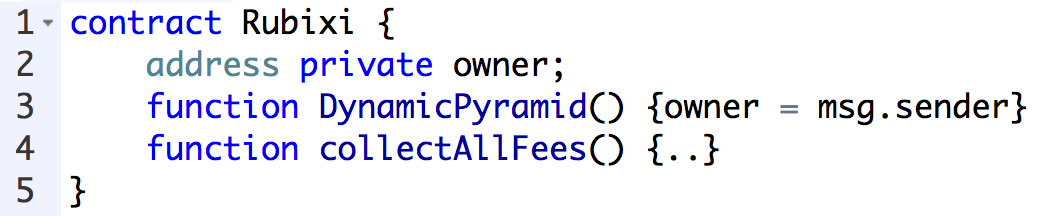
\includegraphics[scale=0.5]{Talk3/img/rubixi2}
\end{center}
\caption{Rubixi Smart Contract}
\label{label}
\end{figure}

This implies that the function at \textit{line 3} called \textit{DynamicPyramid} would have never been able to execute its content and so associate the \textit{owner} of the contract ot the \textit{msg.sender}.

\subsection{Smart contracts make slow Blockchains}
Since every 14 seconds new blocks are mined in \textit{Ethereum} \cite{sina} confirming a set of transactions in a specific order \cite{challenge3}, the blockchain should be a responsive technology in order to elaborate the blocks and validate its execution. \\
However, smart contracts can only be executed in a sequential procedure \cite{challenge3} in order to provide its correct result. This because the transactions's order might affect the outcome. You can consider the block containing this set of transactions as a calculator \cite{challenge1}. If you have to compute some basic operations, like for example 20 divided by 5 substract 2, the correct result will be 2. However, if the order of these operations cannot be guaranteed, another potential result may be 7.3 (20 divided by 5 minus 2). 
You can imagine that there is an analogy between operations and incoming transactions. If the order of two incoming transactions within a block on the blockchain may be reversed or the second one early processed, the execution of the smart contract may be error-prone. \\
This kind of process, which doesn't allow parallel processing can cause some nodes backlogs and so implies delays in the smart contract execution \cite{challenge1}. \\
Indeed, on \textit{Ethereum} if a miner may not able to compute its content in a reasonable time before a new block comes, the whole block execution may be damaged \cite{challenge1}. \\
Since, as mentioned before, every 12 seconds a new block comes in \textit{Ethereum}, the risk of losing some information or that a node drown under a backlog of work\footnote{accumulation over time of work waiting to be done or orders to be fulfilled \cite{challenge4}} is relatively high.

\subsection{Execution of transaction not set in stone}
As we have seen in some attacks, miners are sometimes free to chose what to do. This means that even though a user attaches a high fee to his transaction, it might still be ignored by miners and thus not validated and executed.\\
Due to this problem, some applications of smart contracts in other context may not be possible.


\begin{thebibliography}{99}
\bibitem{ethereum1}\emph{Ethereum Homestead Release.} \url{https://www.ethereum.org} (last accessed March 2017)
\bibitem{wikipedia1}\emph{Blockchain} Wikipedia: \url{https://en.wikipedia.org/wiki/Blockchain} (last accessed February 2017)
\bibitem{blockchain1}\emph{Know More About Blockchain.} \url{https://letstalkpayments.com/an-overview-of-blockchain-technology/} (last accessed March 2017)
\bibitem{blockchain2}\emph{Blockchain Use Cases Part II.} \url{https://letstalkpayments.com/blockchain-use-cases-part-ii-non-financial-and-financial-use-cases/} (last accessed March 2017)


\bibitem{paper1}Loi Luu, Duc-Hiep Chu, Hrishi Olickel, Prateek Saxena, Aquinas Hobor: \emph{Making Smart Contracts Smarter.}. October 2016. \url{http://delivery.acm.org/10.1145/2980000/2978309/p254-luu.pdf?ip=195.176.96.218&id=2978309&acc=ACTIVE\%20SERVICE&key=FC66C24E42F07228\%2EA04051DB0C098788\%2E4D4702B0C3E38B35\%2E4D4702B0C3E38B35&CFID=926344688&CFTOKEN=88107312&__acm__=1492712435_d0f0d96ea04f8cf077c9b90253210778} (last accessed February 2016)

\bibitem{paper2}Atzei, Nicola and Bartoletti, Massimo and Cimoli, Tiziana: \emph{A survey of attacks on Ethereum smart contracts.} 2016. Cryptology ePrint Archive: Report 2016/1007, https://eprint. iacr. org/2016/1007 \url{https://eprint.iacr.org/2016/1007.pdf} (last accessed February 2017)


\bibitem{paper3}Delmolino \textit{et al.}: \emph{Step by Step Towards Creating a Safe Smart Contract: Lessons and Insights from a Cryptocurrency Lab.} 2016.  \url{http://fc16.ifca.ai/bitcoin/papers/DAKMS16.pdf} (last accessed March 2017)




\bibitem{blockchain3}Investopedia: \emph{What is a Blockchain.} \url{http://www.investopedia.com/terms/b/blockchain.asp} (last accessed March 2017)

\bibitem{blockchain4}\emph{Blockchain technology: 9 benefits and 7 challenges.} \url{https://www2.deloitte.com/nl/nl/pages/innovatie/artikelen/blockchain-technology-9-benefits-and-7-challenges.html} (last accessed March 2017)

\bibitem{blockchain5}Hasse, von Perfall, Hillebrand, Smole, Lay, Charlet: \emph{Blockchain - an opportunity for energy producers and consumers?.}\url{http://www.pwc.ch/en/2017/pdf/pwc_blockchain_opportunity_for_energy_producers_and_consumers_en.pdf} (last accessed March 2017)

\bibitem{blockchain6}\emph{What is Blockchain Technology?.} \url{https://blockgeeks.com/guides/what-is-blockchain-technology/} (last accessed March 2017)
\bibitem{blockchain7}\emph{Know More About Blockchain.} \url{https://letstalkpayments.com/an-overview-of-blockchain-technology/} (last accessed April 2017)
\bibitem{blockchain8}\emph{Five Blockchain Applications That Are Shaping Your Future.}\url{http://www.huffingtonpost.com/ameer-rosic-/5-blockchain-applications_b_13279010.html} (last accessed March 2017)
\bibitem{blockchain9}\emph{Future of Blockchain.} \url{https://www.shapingtomorrow.com/home/alert/665529-Future-of--Blockchain} (last accessed February 2017)
\bibitem{blockchain10}\emph{The blockchain problem is a trust problem.}\url{http://usblogs.pwc.com/emerging-technology/the-blockchain-problem-is-a-trust-problem/} (last accessed February 2017)
\bibitem{blockchain11}\emph{How secure is blockchain?.} \url{https://www.taylorwessing.com/download/article-how-secure-is-block-chain.html} (last accessed March 2017)
\bibitem{SC1}\emph{Simple introduction to smart contracts on a blockchain.} \url{https://www.youtube.com/watch?v=FkeLDPZ-v8g&t=134s} (last accessed March 2017)
\bibitem{SC2}\emph{A gentle introduction to smart contracts.} \url{https://bitsonblocks.net/2016/02/01/a-gentle-introduction-to-smart-contracts/} (last accessed February 2017)
\bibitem{SC3}\emph{Blockchain Pros Debate Looming Challenges for Smart Contracts.} \url{http://www.coindesk.com/blockchain-smart-contracts-looming-challenges/} (last accessed April 2017)



\bibitem{blockchain0}Morabito: \emph{Blockchain Value System.} 2017. \url{http://www.springer.com/cda/content/document/cda_downloaddocument/9783319484778-c2.pdf?SGWID=0-0-45-1599947-p180347565} (last accessed March 2017)



\bibitem{SC6}\emph{A USD 50 Million Hack Just Showed That the DAO Was All Too Human}\url{https://www.wired.com/2016/06/50-million-hack-just-showed-dao-human/} (last accessed March 2017)

\bibitem{SC7}\emph{title.}\url{http://www.clydeco.com/insight/article/ethereums-dao-attack-smart-contracts-and-blockchain-face-their-first-big-te} (last accessed April 2017)
\bibitem{SC8}\emph{Ethereum's DAO attack: smart contracts and blockchain face their first big test}\url{http://www.clydeco.com/insight/article/ethereums-dao-attack-smart-contracts-and-blockchain-face-their-first-big-te} (last accessed April 2017)
\bibitem{SC9}\emph{Digital currency Ethereum is cratering because of a USD 50 million hack}\url{http://uk.businessinsider.com/dao-hacked-ethereum-crashing-in-value-tens-of-millions-allegedly-stolen-2016-6} (last accessed April 2017)


\bibitem{SC10}\emph{GitHub: FAQ}\url{https://github.com/chriseth/solidity-doc-test/blob/master/docs/frequently-asked-questions.rst} (last accessed April 2017)




\bibitem{SC11}\emph{What is the "Gas" in Ethereum?}\url{https://www.cryptocompare.com/coins/guides/what-is-the-gas-in-ethereum/} (last accessed March 2017)

\bibitem{SC12}\emph{Wikipedia: Contract}\url{https://en.wikipedia.org/wiki/Contract} (last accessed April 2017)
\bibitem{SC13}\emph{Legally Binding: defintion}\url{http://www.businessdictionary.com/definition/legally-binding.html} (last accessed March 2017)


\bibitem{rubixi1}\emph{Bitcointalk:Hi!MynameisRubixi.}\url{https://bitcointalk.org/index.php?topic=1400536.60} (last accessed April 2017)
\bibitem{rubixi2}\emph{Etherscan: Rubixi code.}\url{https://etherscan.io/address/0xe82719202e5965Cf5D9B6673B7503a3b92DE20be} (last accessed February 2017)
    
    
\bibitem{ponzi}\emph{Schema Ponzi.}\url{https://it.wikipedia.org/wiki/Schema_Ponzi} (last accessed April 2017)
\bibitem{challenge1}\emph{Five Challenges Facing Your Smart Contract Project.}\url{https://makebitcoingreatagain.wordpress.com/2016/02/10/5-challenges-facing-smart-contracts/} (last accessed March 2017)

\bibitem{challenge2}\emph{Thinking About Smart Contract Security.}\url{https://blog.ethereum.org/2016/06/19/thinking-smart-contract-security/} (last accessed April 2017)
\bibitem{vitalin}\emph{Wikipedia: Vitalik Buterin.}\url{https://en.wikipedia.org/wiki/Vitalik_Buterin} (last accessed March 2017)


\bibitem{sina}\emph{Bruno Rodrigues, Thomas Bocek, David Hausheer, Andri Lareida, Sina Rafati, Burkhard Stiller. A Blockchain-based Architecture for Collaborative DDoS Mitigation with Smart Contracts and SDN. 11th International Conference on Autonomous Infrastructure, Management and Security (AIMS 2017). July 10-14, Zurich, Switzerland. To appear.} (last accessed April 2017)

\bibitem{challenge3} Gideon Greenspan. \emph{Smart contracts make slow blockchains.}\url{http://www.multichain.com/blog/2015/11/smart-contracts-slow-blockchains/} (last accessed March 2017)


\bibitem{challenge4}\emph{Wikipedia: Backlog.}\url{https://en.wikipedia.org/wiki/Backlog} (last accessed April 2017)


\bibitem{anal}\emph{Scanning Live Ethereum Contracts for the "Unchecked-Send" Bug.}\url{http://hackingdistributed.com/2016/06/16/scanning-live-ethereum-contracts-for-bugs/} (last accessed March 2017)
\bibitem{SC24}\emph{title.}\url{url} (last accessed April 2017)



\bibitem{timmedCommitments1}\emph{Financial Cryptography and Data Security.}\url{https://books.google.ch/books?id=7YGBCgAAQBAJ&pg=PA14&lpg=PA14&dq=timed+commitments+blockchain&source=bl&ots=jpTIFT8fFx&sig=x9lTOEaQH5K1aU8ipaj1f8dTSO8&hl=it&sa=X&ved=0ahUKEwiWraz8x-rSAhVG72MKHZZ6A7gQ6AEIJTAB#v=onepage&q=timed&f=false} (last accessed Mai 2017)


\bibitem{hardfork}\emph{Announcement of imminent hard fork for EIP150 gas cost changes.}\url{https://blog.ethereum.org/2016/10/13/announcement-imminent-hard-
fork-eip150-gas-cost-changes/} (last accessed Mai 2017)

\bibitem{BlockProtocol}\emph{Block Protocol 2.0.}\url{https://github.com/ethereum/wiki/wiki/Block-Protocol-2.0#block-validation-algorithm} (last accessed Mai 2017)

\bibitem{BitcoinsPriceCharts}\emph{Bitcoins price chart history}\url{https://99bitcoins.com/price-chart-history/} (last accessed Mai 2017)









\end{thebibliography}
